\documentclass[report.tex]{subfiles}
\begin{document}
\newpage
\chapter{INTRODUCTION}
    % what is the program
    Logic circuits are one of the core components of CPUs. These circuits allow manipulating binary data and carrying out various logical operations.
    Programs such as Proteus and Logisim can be used to simulate logic circuits.
    For our project, we decided to create a similar (albeit heavily simplified) logic simulator named \textbf{MinimaLogic}.
    \\\\
    \textbf{MinimaLogic} is a GUI based logic simulator that allows simulation of various logic gates and circuits.
    It allows users to create and simulate circuits ranging from a simple 1-bit adder to more complex circuits like 4-bit counters.
    In fact, one could create any circuit that fits within the available area using the components provided in the program.
    The program allows the user to interact via mouse and keyboard. To make the program user friendly, we tried to keep the controls as intuitive as possible.
    \\\\
    This program heavily relies on the Simple DirectMedia Layer(SDL2) Library for GUI elements as well as user interation/input. 
    Alongside SDL2, the program also utilizes SDL2\_ttf for font rendering as well as the Windows API for opening/saving files.
    Other standard headers that are available with all modern development environments have also been used.
    % describe a little bit about C
    \section{The C Programming Language}
    C is a general-purpose, procedural computer programming language which was developed by Dennis Ritchie in Bell Laboratories between 1972 and 1973 AD as a successor to Basic Combined Programming Language (BCPL or the B language).
    C was designed such that code written in C can be translated efficiently into machine level instructions. 
    Code written in C somewhat resembles the english language as it uses keywords such as \texttt{if, else, for, do}, etc.
    Along with its speed and syntax, C contains addidtional features which allow it to work at lower level thus it can bridge the gap between machine level and high level languages.
    Due to this, C has found lasting use in systems programming (e.g writing operating systems). 
    It can also be used for applications programming. Applications made in C are generally much faster and efficient than most other programming languages even with less optimization.
    \\\\
    Some characteristics of the C language:
    \begin{itemize}
        \item{The language has a small, fixed number of keywords (only 32), including a full set of control flow primitives: if/else, for, do/while, while, and switch.}
        \item{It has a rich set of operators (arithmetic, bitwise, relational, logical and some miscellaneous operators).}
        \item{It allows users to define functions that return value of certain data type however, value returned by function can be ignored if not needed.}
        \item{It also allows for procedures i.e. functions not returning values, by using a return type \texttt{void}.}
        \item{It is a statically typed language i.e. all data has a type, but implicit conversions are possible.}
        \item{Declaration syntax mimics usage context. For eg: C has no "define" keyword; instead, a statement beginning with the name of a type is taken as a declaration.}
        \item{It allows for user-defined (\texttt{typedef}) and compound data types through \texttt{struct}(structure, heterogeneous aggregate data type), \texttt{union}(structure with overlapping members), \texttt{enum}(enumerated data type) and arrays(homogeneous aggregate of data).}
        \item{It allows low-level access to computer memory by converting machine addresses to typed pointers.}
        \item{A preprocessor performs macro definition, source code file inclusion, and conditional compilation.}
        \item{There is a basic form of modularity: files can be compiled separately and linked together, with control over which functions and data objects are visible to other files via \texttt{static} and \texttt{extern} attributes.}
        \item{The standard library of C provides a rich set of functions which allow for complex functionality such as I/O, string manipulation, and mathematical functions.}
    \end{itemize}
    % describe program structure
    \section{Structure of Code}
    Generally, a C program is divided into following sections:
    \begin{itemize}
        \item{Inclusion / Linking Section}\\
            This section consists of header files to be included in the program. Inclusion of files is done using the \texttt{\#include} preprocessor directive. It provides instructions to the compiler to link functions, structures, enums etc. from the header file.
        \item{Macro Definition Section}\\
            This sections consists of macro (or symbolic constants) definitions. Macros are defined using the \texttt{\#define} preprocessor directive. 
        \item{Function Definition Section}\\
            This section consists of definitions of all user defined funtions that are to be used in the program to perform. These functions are called from the \texttt{main()} function.
        \item{Main Function Section}\\
            There can only be one \texttt{main()} function in the entire C program. The \texttt{main()} function acts as the entry point to the program i.e. execution of program begins from the main function.
    \end{itemize}
    \subsection*{Sample C Program}
\begin{lstlisting}
// Linking section
#include <stdio.h>
// Here, the C standard library stdio.h (standard input output) has been included

//Macro definition section
#define MSG "Hello, Peter\n"
//Here, a macro MSG has been defined which expands to "Hello, Peter\n"

//Function definition section
void PrintMessage(){
    printf(MSG);
}
//Here, a function PrintMessage() has been defined
//It calls the printf() function from stdio.h to display value of MSG to the screen

//Main Function Section
int main(){
    PrintMessage();
    return 0;
}
//Here, the main function has been defined which calls the PrintMessage() function defined previously.

// Output
// Hello, Peter
\end{lstlisting}
    The source code for our program has been divided into 9 files (4 headers and 5 C files). Our source code mostly follows this format however at certain parts of the code the format has not been followed for the sake of convinience.
    \begin{figure}[H]
        \centering
        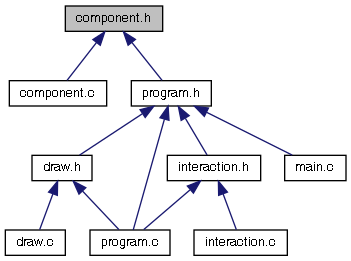
\includegraphics[width=4in]{graphics/component_8h__dep__incl.png}
        \caption{File inclusion graph}
    \end{figure}
    The files are linked as shown in figure above. Other header files have also been linked which is discussed in the implementation section. Functions, structs and enums shared across multiple files have been defined in the relevant header file.
    % describe a little about SDL
    % SDL program loop
    \section{Simple DirectMedia Layer(SDL2)}
    Simple DirectMedia Layer is a cross-platform development library designed to pro-
    vide low level access to audio, keyboard, mouse, joystick, and graphics hardware
    via OpenGL and Direct3D. It is used by video playback software, emulators, and
    popular games including Valve’s award winning catalog and many Humble Bundle
    games.\\\\
    SDL2 libraries also contains extension to keep SDL as light as possible. Some of the
    libraries are SDL2\_image, SDL2\_net, SDL2\_mixer, SDL2\_ttf, true type SDL2\_rtf. SDL2\_image
    is used to load different images, SDL2\_net is used for cross platform networking,
    SDL2\_mixer is an audio mixer library that supports WAV, MP3, MIDI and OGG.
    SDL2\_ttf is used to write using fonts in the program and SDL2\_rtf is Rich Text Format
    library. Out of these libraries, we only used SDL2\_ttf.
    \\\\
    The SDL2 library is more oriented towards game development and it provides a vast quantity of features such as 3D rendering, hardware accelerated 2D graphics, multiple windows, multiple audio devices, multiple input devices etc. 
    Since our program is much simpler than a full fledged game, we were only able to utilize a small fraction of SDL's features.
    \\\\
    SDL programs run continuously in a loop which is often referred to as the game loop. The loop can be summarized by the following diagram:
    \begin{figure}[H]
        \centering
        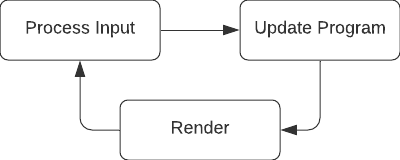
\includegraphics[width=3in]{graphics/SDL_loop.png}
        \caption{SDL program loop}
    \end{figure}
    \subsection*{Sample SDL Program}
    \begin{lstlisting}
// This programs opens a SDL window which shows a blank screen until the user quits
#include <SDL2/SDL.h>
#include <stdio.h>

// Declare SDL window and renderer
SDL_Window *window;
SDL_Renderer *renderer;

int main(int argc, char ** argv) {
    // Display error and quit program if SDL cannot be initialized
    if (SDL_Init(SDL_INIT_EVERYTHING) != 0) {
        printf("Failed to initialize SDL\n");
        return -1;
    }
    // Create a window
    window = SDL_CreateWindow("Demo", 0, 0, 500, 500, SDL_WINDOW_RESIZABLE);
    // Display error and quit program if window cannot be created
    if (!window) {
        printf("Could not create a window: %s", SDL_GetError());
        return -1;
    }
    // Create a renderer
    renderer = SDL_CreateRenderer(window, -1, SDL_RENDERER_SOFTWARE);
    // Display error and quit program if renderer cannot be created
    if (!renderer) {
        printf("Could not create a renderer: %s", SDL_GetError());
        return -1;
    }
    // Main program loop
    while (true) {
        // Get the next event
        SDL_Event event;
        if (SDL_WaitEventTimeout(&event, 10)) // Wait for event (user input) {
            if (event.type == SDL_QUIT) {
                // Exit loop if user presses quit
                break;
            }
	        /* User Input Processing happens here */
        }
        // Clear the screen
        SDL_SetRenderDrawColor(renderer, 0, 0, 0, 255);
        SDL_RenderClear(renderer);

        /* Rendering/drawing code goes here */
        /* Updating code goes here */

        SDL_RenderPresent(renderer); // Update the screen
        SDL_Delay(10);	// Limit frame rate to reduce CPU load
    }
    // Clean up
    SDL_DestroyRenderer(renderer);
    SDL_DestroyWindow(window);
    SDL_Quit();
    return 0;
}
\end{lstlisting}
\end{document}
